\newpage
\section{Theoretische Grundlagen} \label{infos}
In diesem Kapitel soll eine Übersicht über die wichtigsten theoretischen Grundlagen der Arbeiten gegeben werden. Die relevanten Fachbegriffe werden definiert und eine Herleitung der mathematischen Grundlagen der angewendeten Methoden wird dargestellt. Im folgenden Abschnitt wird auf Straßenverkehrsschilder und den verwendeten Datensatz eingegangen.  Anschließend werden wichtige Aspekte von \ac{NN} und \ac{CNN} erläutert und hergeleitet (Abschnitte \ref{sec:NN} bzw. \ref{sec:CNN}). Abschließend werden die verwendeten Algorithmen zur Visualisierung des Gelernten des \ac{CNN} (Abschnitt \ref{sec:visAlgos}) und die Python Bibliotheken die zum Einsatz kommen \ref{sec:bibs} vorgestellt. 
\subsection{Straßenverkehrsschilder}
In diesem Abschnitt soll eine kurze Definition von Straßenverkehrsschilder so wie eine Vorstellung der in Deutschland geltenden Rechtslage dieser gegeben werden. Außerdem wird ein Überblick, über verfügbare Datensätze mit Schwerpunkt auf den \ac{GTSRB} Datensatz gegeben.

\subsubsection{Straßenverkehrsschilder in Deutschland}
Straßenverkehrsschilder dienen dazu, den Straßenverkehr zu regeln. Hierbei stellen sie den Verkehrsteilnehmern Warnungen, Informationen und Einzelheiten über Einschränkungen zur Verfügung. Sie fallen dabei unter die Straßenausstattung und werden behördlich angeordnet. \todo{Beleg} Alle gültigen Straßenverkehrsschilder in Deutschland werden in der \ac{StVO} gelistet. Diese wird fortlaufend den aktuellen Gegebenheiten angepasst und durch Novellen aktualisiert. Grundsätzlich basieren die Straßenverkehrsschilder dabei auf dem am 8. November 1968 in Wien beschlossenen \textit{Übereinkommen über den Straßenverkehr} (engl. Originaltitel "Convention on Road Traffic").\footcite[Vgl.][o.S.]{unConventionRoadTraffic1977} 
 Dieses wurde bis heute von 36 Nationen unterzeichnet und von 84 Nationen ratifiziert.\footcite[Vgl.][1-14]{unUnitedNationsTreaty2020}

In der \ac{StVO} sind drei Gruppen von Verkehrszeichen definiert:
\begin{itemize}
    \item Gefahrenzeichen (§ 40 \ac{StVO})
    \item Vorschriftzeichen (§ 41 \ac{StVO})
    \item Richtzeichen (§ 42 \ac{StVO})
\end{itemize}

Neben diesen Verkehrszeichen gibt es noch Zusatzzeichen, welche zusammen mit Zeichen aus den genannten Gruppen verwendet werden. Diese sind in § 39 Abs. 7 \ac{StVO} aufgelistet.


\subsubsection{German Traffic Sign Recognition Benchmark}
Für den praktischen Teil dieser Arbeit, wird ein Datensatz von Straßenverkehrsschildern benötigt, mit denen das \ac{CNN} initial trainiert und bewertet werden kann. Es gibt eine Vielzahl von Datensätzen die hierfür potentiell geeignet wären. Das \textit{\ac{MASTIF}} Projekt stellt drei verschiedene Datensätze aus den Jahren 2009, 2010 und 2011 zur Verfügung. Der umfangreichste ist hierbei der Datensatz aus 2009 mit 6000 Bildern.\footcite[Vgl.][S. 66-73]{vsegvic2010computer} Shakhuro und Konushin stellen einen Datensatz mit 104.358 verschiedenen russischen Schildern aus dem Jahre 2016 zur Verfügung.\footcite[Vgl.][S. 294-300]{rtsd} Der bisher umfangreichste Datensatz ist das \textit{Mapillary Traffic Sign Dataset} aus dem Jahre 2020. Es enthält 100.000 Bilder mit insgesamt 325.172 erkannten Schildern. Von diesen Schildern Fallen 82.724 Schilder in die im Datensatz gekennzeichneten Schilderklassen. Die Bilder stammen dabei aus der ganzen Welt, eine grobe Verteilung liegt bei 20\% Nordamerika, 20\% Europa, 20\% Asien, 15\% Südamerika, 15\% Ozeanien und 10\% Afrika.\footcite[Vgl.][S. 1-17]{ertlerMapillaryTrafficSign2020}

\begin{table}[t]
    
    \caption{Übersicht der höchsten erreichten Genauigkeiten auf den GTSRB Datensatz\label{table:TopGTRSBPaper}}
    \resizebox{\textwidth}{!}{%
    \begin{tabular}{@{}llc@{}}
    \toprule
    \textbf{Team}                                        & \textbf{Methode}                                           & \begin{tabular}[c]{@{}c@{}}\textbf{Prozentzahl} \\ \textbf{(Genauigkeit)}\end{tabular} \\ \midrule
    Arcos-García, Álvarez-García, Soria-Morillo & CNN mit 3 Spatial Transformers                    & 99.71                                                                \\
    Ciresan, Meier, Masci, Schmidhuber         & Zusammenschluss mehrerer CNNs                     & 99.46                                                                \\
    Gecer, Azzopardi, Petkov                  & Farbenbasierter COSFIRE-Filterzur Objekterkennung & 98.97                                                                \\
    Stallkamp, Schlipsing, Salmen, Igel & Durchschnittliches menschliches Abschneiden & 98.84 \\
    Sermanet, LeCun                            & Mehrstufige CNNs                                  & 98.31                                                                \\ \bottomrule
    \end{tabular}%
    }
    
    \hfill \break
    Quelle: In Anlehnung an Institut für Neuroinformatik Ruhr-Universität Bochum, Resultate GTSRB, 2019, o.S.
\end{table} 
Letztendlich wurde sich für den Datensatz \ac{GTSRB} entschieden. Dieser umfasst 51.840 Bilder von 1700 verschiedenen deutschen Straßenverkehrsschilder, welche in 43 Klassen unterteilt wurden. Grund für die Auswahl war primär, dass dieser Datensatz die größte Anzahl von deutschen Straßenverkehrsschilder bereitstellt, auf denen  der Schwerpunkt dieser Arbeit liegt. Der Datensatz wurde im Jahre 2010 erstellt und die Maße der Bilder variieren zwischen 15x15 und 222x193 Pixeln. In Abbildung \ref{fig:overviewClassesGTSRB} wird die Anzahl der Bildern pro Klasse im Trainingsdatensatz des \ac{GTSRB} dargestellt. Die 43 Klassen des Datensatzes fallen alle unter die drei Gruppen der Verkehrszeichen nach § 39 Abs. 2 Satz 2 \ac{StVO}. Dabei fallen 27 Klassen unter Vorschriftzeichen, 14 Klassen unter Gefahrenzeichen und 2 Klassen unter Richtzeichen. \todo{Ggf ins Glossar}
Für den \ac{GTSRB} liegen eine Vielzahl von Forschungsarbeiten vor.\footcite[Vgl.][S. 158 - 165]{arcos-garciaDeepNeuralNetwork2018}\footcite[Vgl.][165-174]{gecerColorblobbasedCOSFIREFilters2017}\footcite[Vgl.][S. 333-33]{ciresanMulticolumnDeepNeural2012}\footcite[Vgl.][S. 323-332]{Stallkamp2012}\footcite[Vgl.][S. 2809-2813]{sermanetTrafficSignRecognition2011} Die fünf Einreichungen mit der höchsten \textit{Accuracy} (Genauigkeit) auf dem Testdatensatz sind in Tabelle \ref{table:TopGTRSBPaper} aufgelistet. Es ist zu erkennen, dass bereits eine sehr hohe Accuracy erreicht wird (99.71\%). 


\begin{figure}[t]
    \centering
    \caption[]{Anzahl Bilder pro Klasse im GTSRB Trainingsdatensatz}
	\label{fig:overviewClassesGTSRB}
    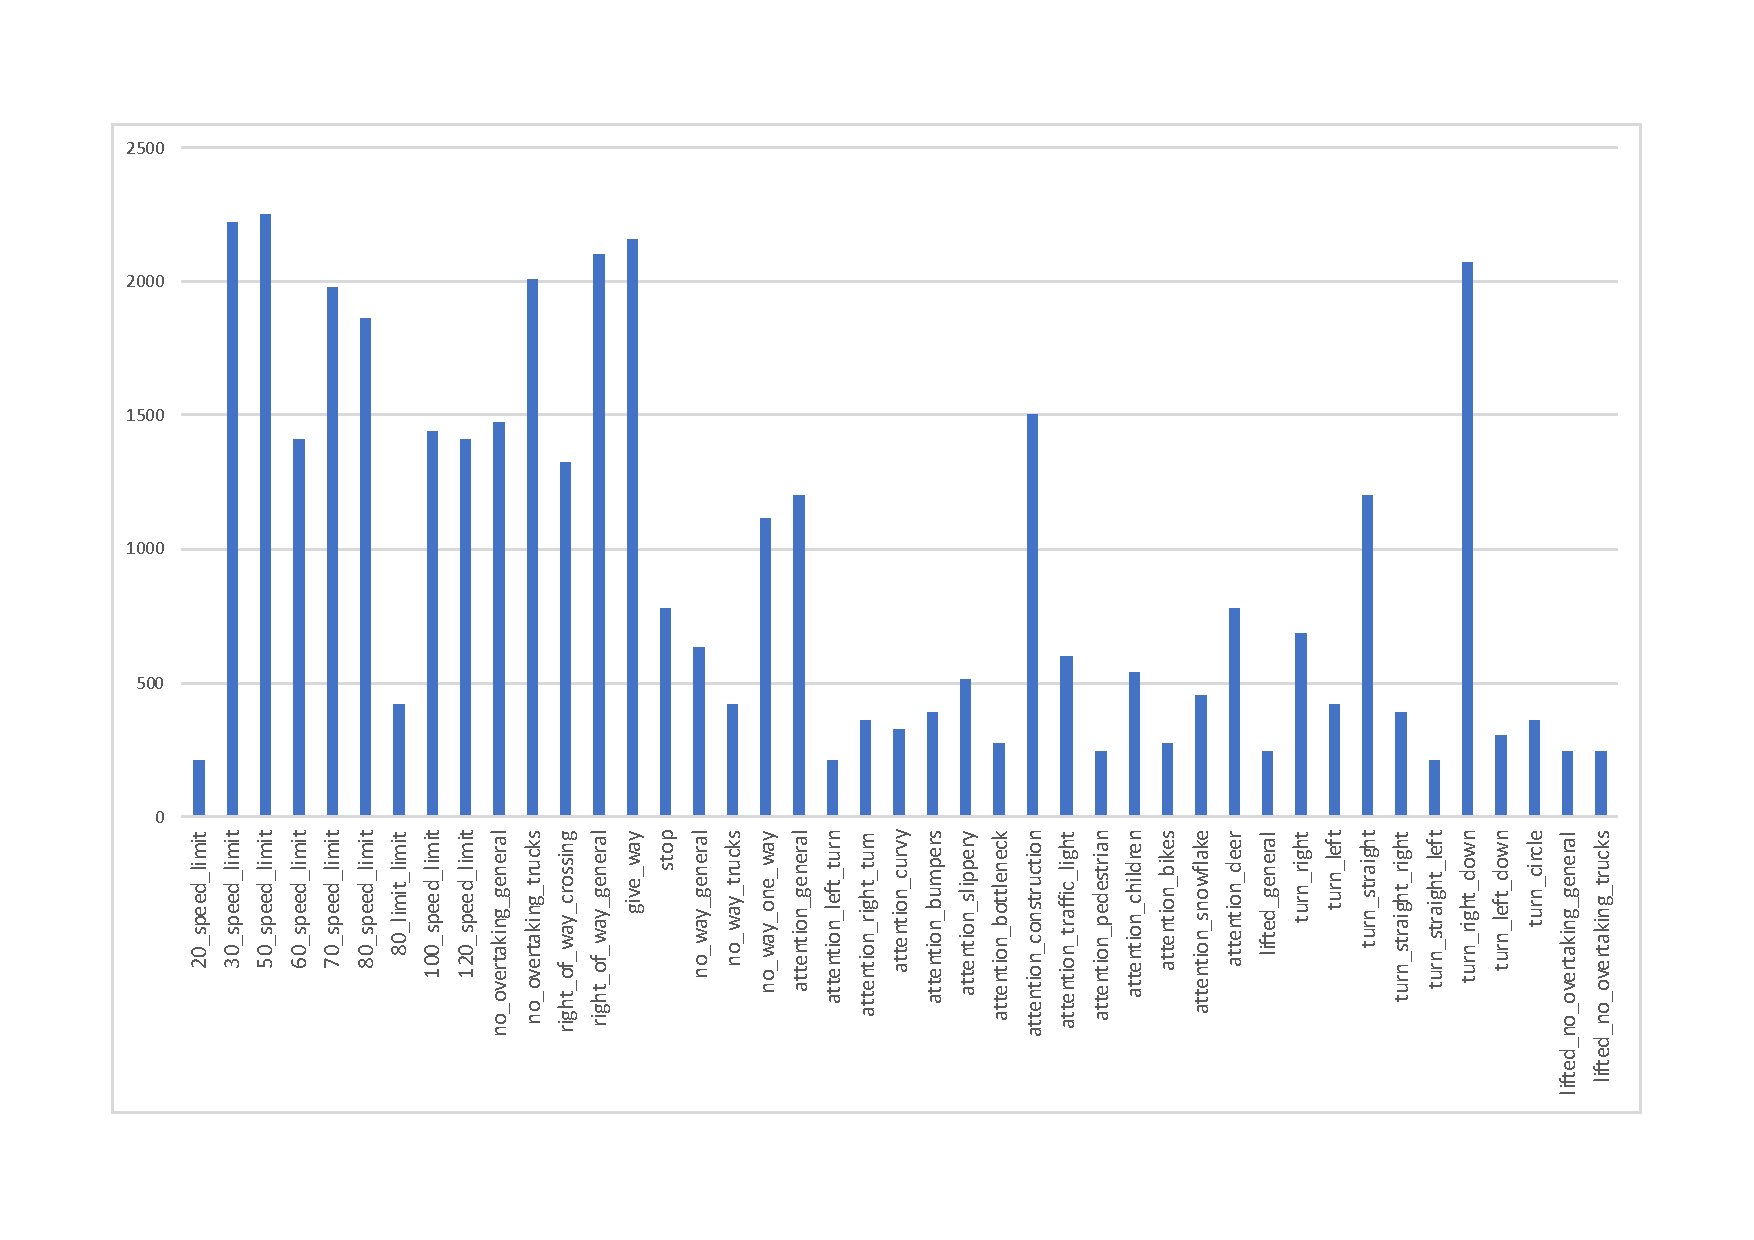
\includegraphics[width=1\textwidth]{image_per_class.pdf}
    Quelle: Eigene Darstellung, 2020
\end{figure}


 

\subsection{Neural Networks} \label{sec:NN}
In den letzten Jahren gab es eine Vielzahl von Fortschritten durch Computersysteme, die durch die Allgemeinheit unter dem Begriff \ac{KI} zusammen gefasst werden. So konnte zum Beispiel AlphaGo einen der weltweit besten Spieler in dem Brettspiel Go schlagen und das System DeepFace ist in der Lage, menschliche Gesichter nahezu auf menschlichen Niveau erkennen zu können.\footcites[Vgl.][]{spiegelGoogleComputerAlphaGo2016}\footcite[Vgl.][]{taigman2014deepface}

Systeme die als \ac{KI} bezeichnet werden, sind häufig in der Lage, Aufgaben zu bewältigen die bisher ausschließlich durch das menschliche Gehirn bearbeitet werden konnten. Neben den oben genannten Beispielen zählt hier auch das Erkennen von Bildern oder Sprache dazu. Damit Computer diese Aufgaben erledigen können, haben Wissenschaftler sich vom menschlichen bzw. biologischen Gehirn inspirieren lassen. Systeme die auf dieser Grundlage basieren und einige der Vorgehensweisen des Gehirnen imitieren, werden als \ac{NN} bezeichnet.

\subsubsection{Aufbau}
Die grundlegenden Bausteine von \ac{NN} sind Perceptron und wurden 1958 von Rosenblatt beschrieben.\footcite[Vgl.][]{rosenblattPerceptronProbabilisticModel1958} Als Grundlage verwendete er hierbei unter anderem die Arbeit von McCulloch und Pitts.\footcite[Vgl.][]{mccullochLogicalCalculusIdeas1943}

\tikzset{%
  neuron missing/.style={
    draw=none, 
    scale=3,
    text height=0.333cm,
    execute at begin node=\color{black}$\vdots$
  },
}

\begin{figure}[t]
	\centering
	\begin{tikzpicture}[x=1.5cm, y=1.5cm,  >=stealth]
        \tikzstyle{unit}=[draw,shape=circle,minimum size=1.2cm]
        \tikzstyle{weight} =[draw, shape=rectangle, minimum size=.8cm]


        \node[unit](x1) at (0,3.5){$I_1$};
        \node[unit](xn) at (0,1.5){$I_{N}$};
        \node(dots) at (0,2.5){\vdots};
        \node[unit](bias) at (0,0){$b$};

        \node[weight](w1) at (2,3){$w_1$};
        \node[weight](wn) at (2,1.5){$w_n$};
        \node[weight](wb) at (2,0.5){$w_b$};

        \node[unit](wSum) at (4,1.5){$\sum$};

        \draw[->] (bias) -- (wb);
        \draw[->] (x1) -- (w1);
        \draw[->] (xn) -- (wn);
        \draw[->] (wb) -- (wSum);
        \draw[->] (w1) -- (wSum);
        \draw[->] (wn) -- (wSum);

        \draw [->] (wSum) -- ++(1,0)
        node [above, midway] {};
        
        \end{tikzpicture}
	\caption[]{Darstellung eines Perceptron}
    \label{fig:perceptron}
    Quelle: Eigene Darstellung, 2020
\end{figure}

Ein Perceptron kann zwischen $1$ und $n$ Eingangssignalen sowie einen negativen Bias Term\footnote{Einige Defintionen schreiben nicht vor, dass der Bias negativ sein muss. Stattdessen wird dieser im weiteren Vorgehen subtrahiert statt summiert zu werden} $b$ erhalten und hieraus ein Ausgangssignal - auch Aktivierung genannt - erzeugen. Für das Ausgangssignal werden alle Eingangssignale jeweils mit einem eigenen - als Gewicht bezeichneten - Faktor multipliziert (siehe Abbildung \ref{fig:perceptron}). Die Ergebnisse werden anschließend zusammen mit dem Bias summiert. Ist die Summe kleiner oder gleich $0$, ist der Ausgangswert ebenfalls $0$, ansonsten beträgt der Ausgangswert $1$. Der Bias stellt also den Schwellwert dar, denn die gewichtete Summe überschreiten muss, damit das Ausgangssignal $1$ lautet. 

Es ist möglich, ein Perceptron um eine Aktivierungsfunktion zu ergänzen, sodass das Ausgabesignal reelle Werte annehmen kann. Diese Erweiterung des Perceptron wird als Neuron bezeichnet. Weit verbreitet ist die Verwendung der Sigmoid Funktion (siehe Gleichung \ref{eq:sigmoid}). Bei der Anwendung einer Aktivierungsfunktion, häufig mit $\sigma$ dargestellt, wird die gewichtete Summe $z$ in die gewählte Funktion gegeben und das Ergebnis stellt das Ausgangssignal des Neuron da (siehe Gleichung \ref{eq:outputNeuron}).

\begin{equation} \label{eq:sigmoid}
    \sigma (z) =  \frac{1}{1+e^{-z}}
\end{equation}

\begin{equation} \label{eq:outputNeuron}
    a = \sigma (\sum_{i}{x_i w_i + b})
\end{equation}

Neben der Sigmoid Funktion werden in modernen \ac{NN} häufig die ReLu Funktion (Gleichung \ref{eq:ReLU}) oder die tanh Funktion (Gleichung \ref{eq:tanh}) verwendet. Alle drei werden in Abbildung \ref{fig:activationfunctions} gegenüber gestellt. Es ist zu erkennen, dass sowohl bei der Sigmoid Funktion, als auch bei der ReLU Funktion die untere Grenze des Wertebereichs bei $0$ liegt. Bei der tanh Funktion, liegt diese bei $-1$. Außerdem haben nur die Sigmoid- und tanh Funktion eine obere Grenze - beide 1 - definiert. ReLU kann jeden Wert größergleich $0$ annehmen. Verwendet man eine Aktivierungsfunktion, stellt der Bias kein Schwellwert mehr dar. Er ist als einziger Term in der Berechnung des Wertes der in die Aktivierungsfunktion gegeben wird von den Eingangswerten unabhängig und sorgt somit um eine konstante Verschiebung.

\begin{equation} \label{eq:ReLU}
    ReLU(z) = max(0,z)
\end{equation}

\begin{equation} \label{eq:tanh}
    \tanh(z) = \frac{\sinh(z)}{\cosh(z)} = \frac {e^z - e^{-z}} {e^z + e^{-z}}
  = \frac{e^{2z} - 1} {e^{2z} + 1}
\end{equation}

\begin{figure}[t]
    \centering
    \caption[]{Darstellung der Sigmoid-, ReLU- und tanh Funktion}
	\label{fig:activationfunctions}
    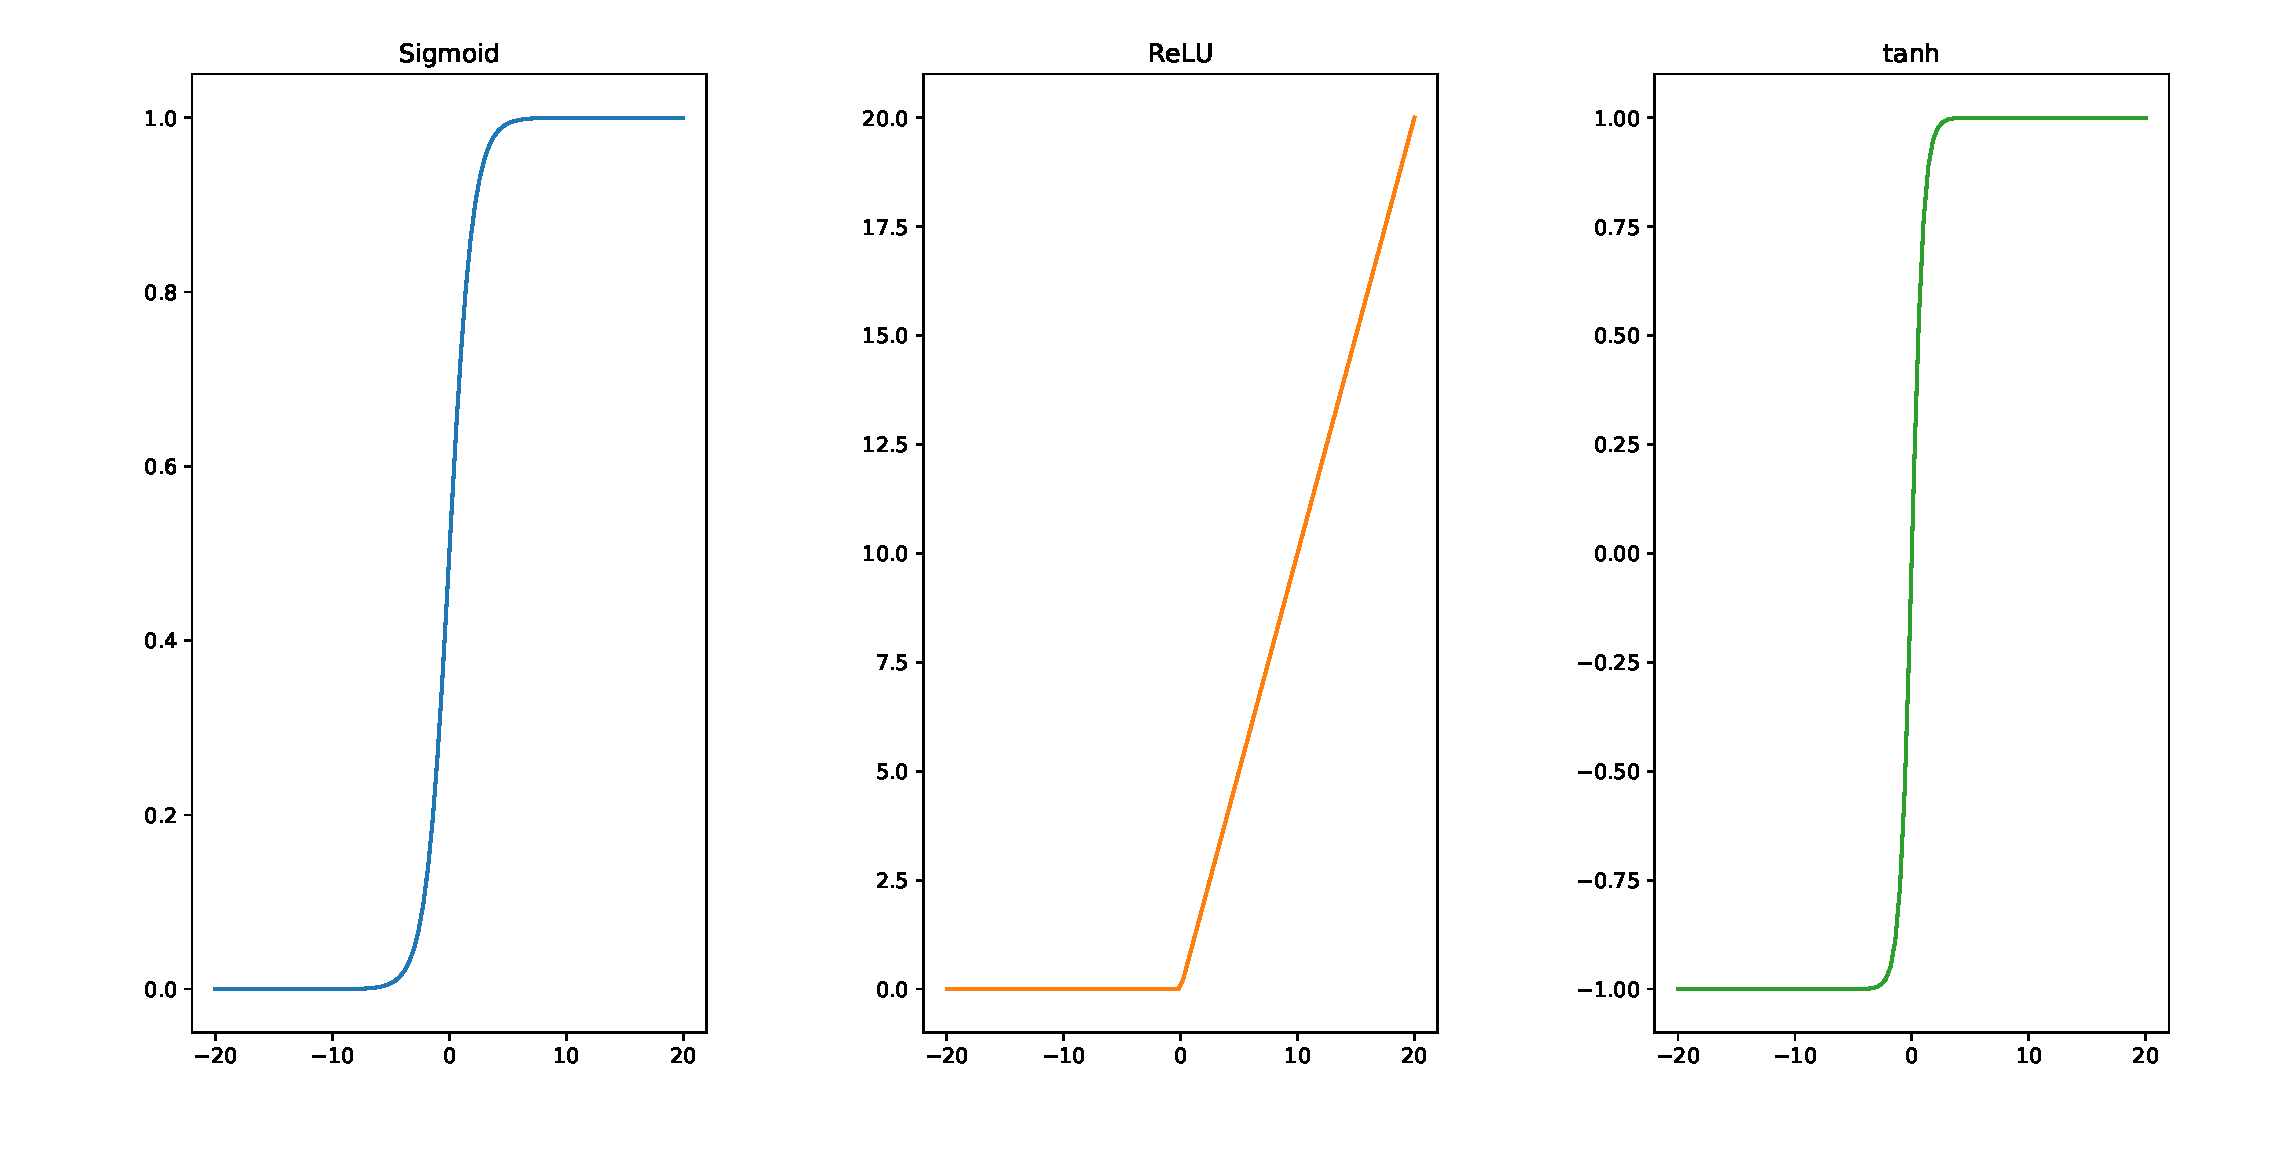
\includegraphics[width=1\textwidth]{activationfunctions.eps}
    Quelle: Eigene Darstellung, 2020
\end{figure}

Ein \ac{NN} besteht aus mehreren, verschalteten Neuronen. Diese werden in Layern angeordnet, welche typischerweise mit $1$ bis $N$ durchnummeriert werden. Layer 1 wird außerdem als Input Layer bezeichnet, da dieser die einzelnen Eingangswerte in das \ac{NN} darstellt. Layer N wiederum wird als Output Layer bezeichnet, da er das Ergebnis des \ac{NN} ausgibt. Alle Layer dazwischen (1 < $l$ < N) werden als Hidden Layer bezeichnet, da von außen weder direkt auf die Eingangssignale der Neuronen in diesen Layern Einfluss genommen werden kann, noch die Ausgabesignale dieser direkt ersichtlich sind. Jeder Layer kann dabei eine unterschiedliche Anzahl von Neuronen enthalten. Typischerweise sind die Neuronen in einem Layer mit allen Neuronen des vorherigen Layers verbunden, ist dies der Fall, wird der Layer auch \textit{Dense Layer} bezeichnet. Eine allgemeine Darstellung eines \ac{NN} mit drei Layern ist in Abbildung \ref{fig:multilayer-perceptron} dargestellt.

\tikzset{%
  every neuron/.style={
    circle,
    draw,
    minimum size=1.2cm
  },
  neuron missing/.style={
    draw=none, 
    scale=3,
    text height=0.333cm,
    execute at begin node=\color{black}$\vdots$
  },
}

\begin{figure}[t]
	\centering
	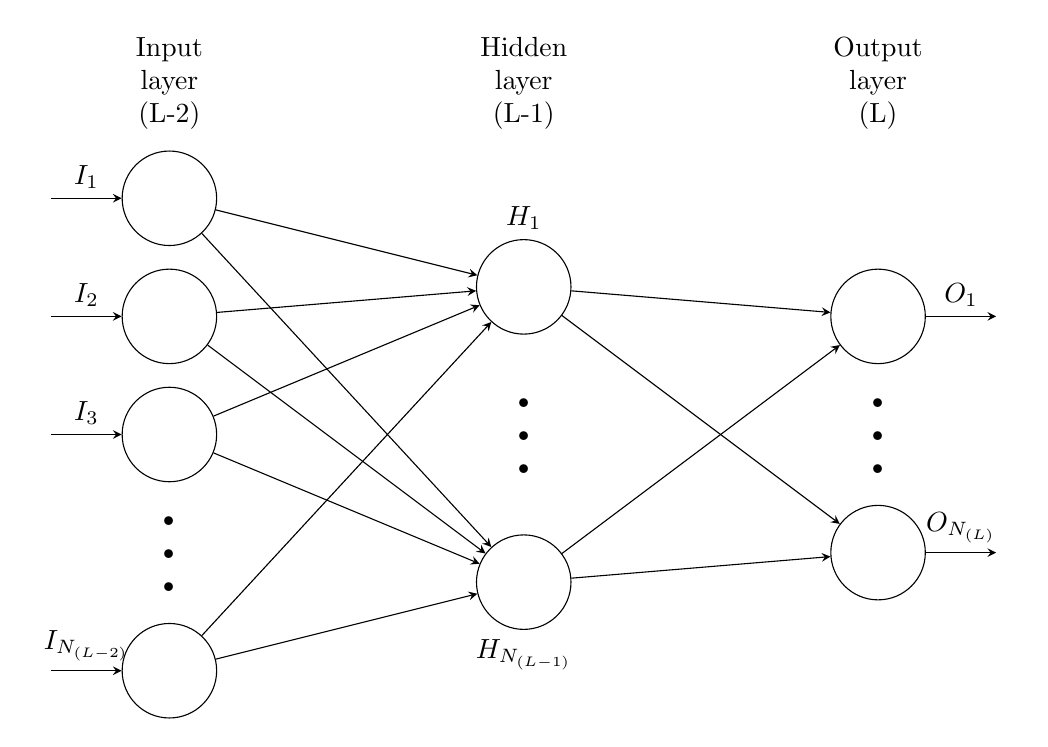
\begin{tikzpicture}[x=1.5cm, y=1.5cm,  >=stealth]

        \foreach \m/\l [count=\y] in {1,2,3,missing,4}
          \node [every neuron/.try, neuron \m/.try] (input-\m) at (0,2.5-\y) {};
        
        
        \foreach \m [count=\y] in {1,missing,2}
          \node [every neuron/.try, neuron \m/.try ] (hidden-\m) at (3,2-\y*1.25) {};
        
        \foreach \m [count=\y] in {1,missing,2}
          \node [every neuron/.try, neuron \m/.try ] (output-\m) at (6,1.5-\y) {};
        
        \foreach \l [count=\i] in {1,2,3}
          \draw [<-] (input-\i) -- ++(-1,0)
            node [above, midway] {$I_\l$};
        \draw [<-] (input-4) -- ++(-1,0)
            node [above, midway] at (input-4) {$I_{N_{(L-2)}}$};
        
        \node [above] at (hidden-1.north) {$H_1$};
        \node [below] at (hidden-2.south) {$H_{N_{(L-1)}}$};
        
        
        \draw [->] (output-1) -- ++(1,0)
        node [above, midway] {$O_1$};
        \draw [->] (output-2) -- ++(1,0)
        node [above, midway] {$O_{N_{(L)}}$};
        
        \foreach \i in {1,...,4}
          \foreach \j in {1,...,2}
            \draw [->] (input-\i) -- (hidden-\j);
        
        \foreach \i in {1,...,2}
          \foreach \j in {1,...,2}
            \draw [->] (hidden-\i) -- (output-\j);
        
        %\foreach \l [count=\x from 0] in {Input, Hidden, Ouput}
        \node [align=center, above] at (0*2,2) {Input \\ layer \\ (L-2)};
        \node [align=center, above] at (1.5*2,2) {Hidden \\ layer \\ (L-1)};
        \node [align=center, above] at (3*2,2) {Output \\ layer \\ (L)};
        
        \end{tikzpicture}
	\caption[]{Allgemein Darstellung eines Neural Network mit 3 Layern}
    \label{fig:multilayer-perceptron}
    Quelle: Eigene Darstellung, 2020
\end{figure}



\subsubsection{Gradient Descent}
Im Rahmen des Lernprozesses eines \ac{NN} werden die Gewichte und Bias der einzelnen Perceptron regelmäßig aktualisiert. Dabei liegt das Ziel darin, durch die Optimierung dieser Faktoren den Fehler des \ac{NN} bei der Vorhersage zu minimieren.

Um diesen Fehler bestimmen zu können, wird eine Verlustfunktion angewendet. Ein einfaches Beispiel einer Verlustfunktion basiert auf der mittleren quadratischen Abweichung.

\begin{equation} \label{eq:mse}
    C(w,b) = \frac{1}{2} \sum (y-\hat{y})^2
\end{equation}

In Gleichung \ref{eq:mse} werden die Gewichte mit \textit{w} und die Bias mit \textit{b} bezeichnet. Zusätzlich werden die wahren Klassen durch \textit{y} und die Ausgabe des \ac{NN} durch \textit{\^{y}} dargestellt. \todo{Prüfen ob variablen konsistent verwendet werden}


Um den Fehler des \ac{NN} zu minimieren, muss der globale Tiefpunkt der Verlustfunktion bestimmt werden. Bei Funktionen mit einer Vielzahl von Parametern, ist es zu komplex, diese Aufgabe analytisch zu lösen. \textit{\ac{GD}} stellt einen iterativen Prozess dar, sich dem nächsten Minimum zu nähern. Bildlich kann dieser Vorgang mit einem Wanderer, der vom Gipfel eines Berges absteigen möchte, verglichen werden. Geht dieser von seinem aktuellen Standpunkt ein paar Schritte in die entgegengesetzte Richtung der steilsten Stelle am Berg und wiederholt diesen Vorgang immer wieder, wandert er immer weiter ins Tal. Betrachtet man Abbildung \ref{fig:quadLoss}, würde der Wanderer in einem der braunen Quadrate beginnen und sich Schritt für Schritt tiefer bis zum blauen Bereich vorarbeiten. 

Mathematisch gesehen kann dies als eine Funktion \textit{L(v)} gesehen werden, wobei \textit{v} eine beliebige Anzahl von Parametern darstellt. Für eine bessere Übersichtlichkeit, wird im folgendem mit zwei Parametern, \textit{v\textsubscript{1}} und \textit{v\textsubscript{2}} gerechnet.

\begin{figure}[t]
    \centering
    \caption[]{Beispiel quadratische Verlustfunktion mit den Parametern v\textsubscript{1} und v\textsubscript{2}}
	\label{fig:quadLoss}
    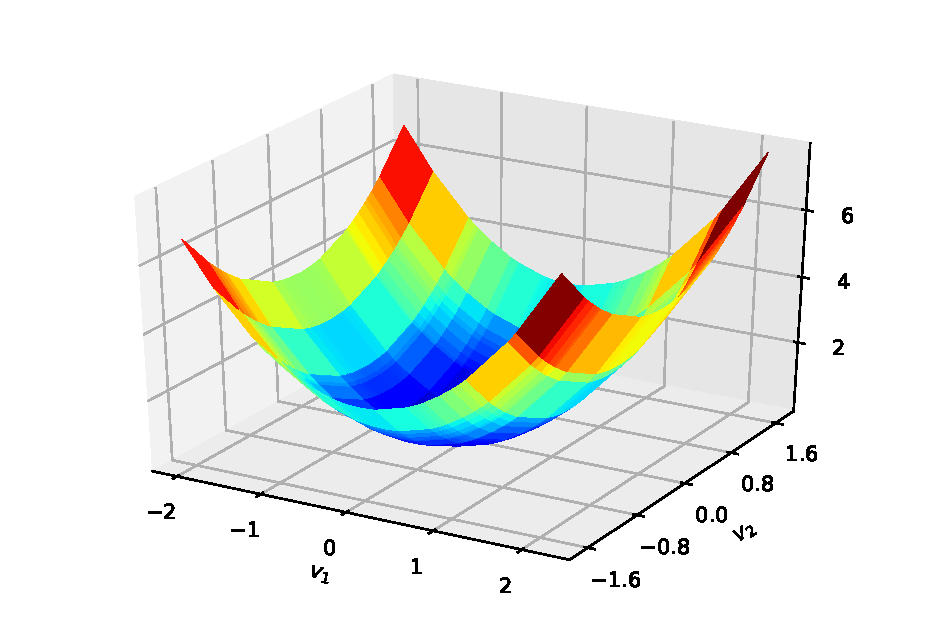
\includegraphics[width=1\textwidth]{quadratic_loss_function.eps}
    Quelle: Eigene Darstellung, 2020
\end{figure}

\begin{equation} \label{eq:deltaL}
    \Delta C \approx \frac{\partial C}{\partial_{v1}} \Delta v_{1} + \frac{\partial C}{\partial_{v2}} \Delta v_{2}
\end{equation}

In Gleichung \ref{eq:deltaL} wird die Funktion $\Delta$L als Summe der partiellen Ableitungen von \textit{v\textsubscript{1}} und \textit{v\textsubscript{2}} definiert. Die hierdurch erhaltenen Gradienten zeigen in die Richtung der größten Änderungen von \textit{v\textsubscript{1}} beziehungsweise \textit{v\textsubscript{2}} .

Fasst man die Parameter \textit{v\textsubscript{1}} und \textit{v\textsubscript{2}} und die partiellen Ableitungen jeweils in einem Vektor zusammen (Gleichung \ref{eq:vector1} und \ref{eq:vector2}), kann Gleichung \ref{eq:deltaL} zu Gleichung \ref{eq:vereinfachung1} umgeformt werden. $\Delta$v kann hierbei als der Vektor der Veränderung der Parameter gesehen werden.

\begin{equation} \label{eq:vector1} 
    \Delta v \equiv \binom{\Delta v_{1}}{ \Delta v_{2}}
\end{equation}

\begin{equation} \label{eq:vector2}
    \nabla C \equiv (\frac{\     C}{\partial_{v1}},  \frac{\partial C}{\partial_{v1}})^{T}
\end{equation}

\begin{equation} \label{eq:vereinfachung1}
    \Delta C \approx \nabla C \cdot \Delta v
\end{equation}

Um den Gesamtverlust zu reduzieren, muss der Vektor $\Delta$v in jedem Durchgang aktualisiert werden. Durch den Gradienten ist die Richtung der größten Änderung vom aktuellen Punkt der Funktion aus bekannt. Da der Gesamtverlust minimiert werden soll, muss in die entgegengesetzte Richtung des Gradienten gegangen werden. Dessen Wert wird also negiert. Außerdem muss eine positive Schrittweite bestimmt werden, die skaliert wie Weit in die Gegenrichtung des Gradienten gegangen wird. Diese wird als \textit{Learning Rate} und häufig mit $\alpha$ bezeichnet. Gleichung \ref{eq:learningRate} zeigt, wie die Veränderung der Parameter, $\Delta$v, mittels $\alpha$ skaliert und das Ergebnis negiert wird.

\begin{equation} \label{eq:learningRate}
    \Delta v = -\alpha \nabla C
\end{equation}      

Wird Gleichung \ref{eq:learningRate} in Gleichung \ref{eq:vereinfachung1} eingesetzt und umgeformt, erhält man Gleichung \ref{eq:finalGradDes}. Da  $\nabla C^2$ und $\alpha$ jeweils positiv sind, ist sichergestellt, dass die vorgenommene Veränderung negativ ist. Dies bedeutet, dass der Verlust mit jedem Durchgang verringert wird. Das \ac{NN} lernt also und seine Ausgaben weichen weniger von den wahren Werten ab. Anzumerken ist hierbei noch, dass das Minimum bei einer zu groß gewählten \textit{Learning Rate} überschritten werden kann. Dies würde dazu führen, dass man den Tiefpunkt überschreitet und wieder ein Stück hoch geht. Außerdem kann das erreichte Minimum ein lokales und nicht globales Minimum sein. Dies ist abhängig vom Startpunkt, da der negierte Gradient immer zum nächstgelegenen Minimum führt.

\begin{equation} \label{eq:finalGradDes}
    \Delta C \approx -\alpha \nabla C \cdot  \nabla C =  -\alpha \nabla C^2
\end{equation}

Ersetzt man \textit{v\textsubscript{1}} und \textit{v\textsubscript{2}} durch \textit{w} und \textit{b}, ist die Berechnung der neuen Werte für die Gewichte \textit{w\textsubscript{j}} und Bias \textit{b\textsubscript{j}} wie in den Gleichungen dargestellt \ref{eq:updateW} und \ref{eq:updateB} definiert.
\begin{equation} \label{eq:updateW}
    w_{j} \rightarrow w_{j}^{'} = w_{j} - \alpha \frac{\partial C}{\partial w_{j}}
\end{equation}

\begin{equation} \label{eq:updateB}
    b_{j} \rightarrow b_{j}^{'} = b_{j} - \alpha \frac{\partial C}{\partial b_{j}}
\end{equation}

\textit{\ac{GD}} betrachtet alle Beispiele im Trainingsdatensatz, bevor die Gewichte und Bias das erste Mal angepasst werden. Da dies  besonders bei großen Trainingsdatensätzen sehr zeit- und rechenintensiv ist, wird bei diesen Datensätzen häufig \ac{SGD}\footcite[Vgl. ][S. 400 ff.]{robbinsStochasticApproximationMethod1951}  angewendet. Bei \ac{SGD} werden die Anpassungen bereits nach einem oder einer Gruppe von Beispielen aus dem Datensatz durchgeführt. Dies hat zwar den Nachteil, dass die Optimierung der Verlustfunktion schlechter sein kann als bei \ac{GD}, allerdings konvergiert \ac{SGD} meistens schneller.

\subsubsection{Backpropagation}

Wie im letzten Abschnitt beschrieben, müssen für die Anwendung von \ac{GD}  $\frac{\partial C}{ \partial w}$ und  $\frac{\partial C}{ \partial b}$ berechnet werden. Rumelhart et al. haben für eine schnelle und effiziente Berechnung dieser im Jahr 1986 den Backpropagation Algorithmus vorgeschlagen.\footcite[Vgl. ][S. 533 ff.]{rumelhart1986learning} Dieser stellt eine erweiterung der Delta-Regel auf \ac{NN} mit mehr als zwei Schichten dar.\todo[]{Quelle einfügen} Die Grundidee besteht darin, den Fehler des \ac{NN} auf die einzelnen Gewichte und Bias innerhalb des \ac{NN} zurückzuführen, so dass diese angepasst werden können. 
%Im folgenden wird primär auf die Gewichte eingegangen, da die Berechnung für einen Bias als einfachere Form der Rechnung für Gewichte angesehen werden kann. 
Formuliert man die Grundidee zum Beispiel für die Gewichte um, stellt sich die Frage, in wie sehr sich der Fehler des \ac{NN} ändert, wenn das Gewicht $w_{jk}$ angepasst wird (siehe Gleichung \ref{eq:defDeltaEdef}).

\begin{equation} \label{eq:defDeltaEdef}
    \frac{\partial C}{ \partial w_{jk}}
\end{equation}

\begin{figure}[t]
	\centering
	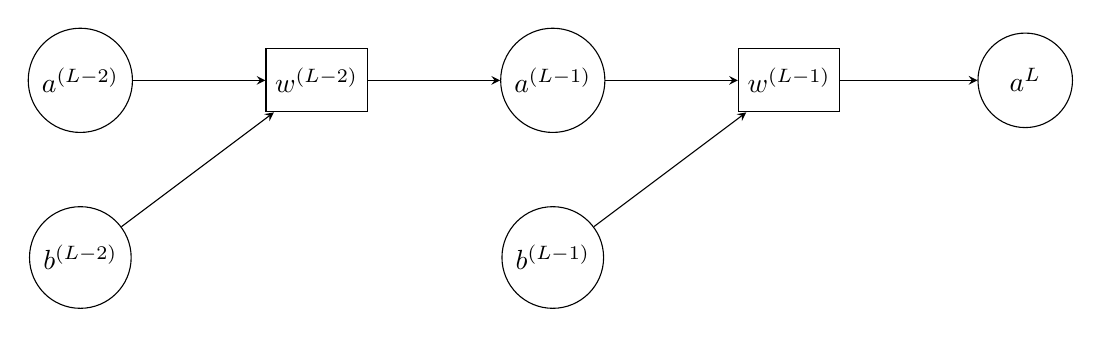
\begin{tikzpicture}[x=1.5cm, y=1.5cm,  >=stealth]
        \tikzstyle{unit}=[draw,shape=circle,minimum size=1.2cm]
        \tikzstyle{weight} =[draw, shape=rectangle, minimum size=.8cm]

        \node[unit](I) at (0, 2){$a^{(L-2)}$};
        \node[unit](b1) at (0,0.5){$b^{(L-2)}$};
        \node[weight](w1) at (2,2){$w^{(L-2)}$};
        \node[unit](H) at (4, 2){$a^{(L-1)}$};
        \node[unit](b2) at (4,0.5){$b^{(L-1)}$};
        \node[weight](w2) at (6,2){$w^{(L-1)}$};
        \node[unit](O) at (8, 2){$a^L$};
        
        \draw[->] (I) -- (w1);
        \draw[->] (w1) -- (H);
        \draw[->] (H) -- (w2);
        \draw[->] (w2) -- (O);
        \draw[->] (b1) -- (w1);
        \draw[->] (b2) -- (w2);
        
        \end{tikzpicture}
	\caption[]{Einfaches Neural Network mit nur einem Neuron pro Layer}
    \label{fig:simpleNetwork}
    Quelle: Eigene Darstellung, 2020
\end{figure}


\begin{figure}[t]
    \centering
    \begin{tikzpicture}[x=1.5cm, y=1.5cm,  >=stealth]
        \tikzstyle{unit}=[draw,shape=circle,minimum size=1.2cm]
        \tikzstyle{weight} =[draw, shape=rectangle, minimum size=.8cm]

        \node[weight](w) at (0, 2){$w^{(L-1)}$};
        \node[weight](a) at (0, 1){$a^{(L-1)}$};
        \node[weight](b) at (0,0){$b^{(L-1)}$};
        \node[weight](z) at (2, 1){$z^{(L)}$};
        \node[weight](aL) at (4,1){$a^{(L)}$};
        \node[unit](c) at (6,1){$C$};
        \node[weight](y) at (6,0){$y$};

        \draw[->] (w) -- (z);
        \draw[->] (a) -- (z);
        \draw[->] (b) -- (z);
        \draw[->] (z) -- (aL);
        %\path [line] (aL) -- node [text width=2.5cm,midway,above ]{$\hat{y}$} (c);
        \draw[->] (aL) -> node [text width=2.5cm,midway,above,align=center ] {$\hat{y}$} (c);

        \draw[->] (y) -- (c);

        \end{tikzpicture}
    \caption[]{Explizite Darstellung Einflüsse der Verlustfunktion des Output Layers}
    \label{fig:unfoldedCost}
    Quelle: Eigene Darstellung, 2020
\end{figure}

Stellt man sich ein möglichst einfaches \ac{NN} mit Hidden Layer vor, erhält man das in Abbildung \ref{fig:simpleNetwork} dargestellte \ac{NN}. Dieses enthält pro Layer nur ein Neuron sowie einen Bias. Alle Gewichte eines Layers wurden für eine bessere Übersichtlichkeit als ein Element repräsentiert. Das heißt, $w^{(L-n)}$ stellt jeweils einen Vektor mit zwei Elementen dar. $a^{L}$ bzw. $a^{(L-n)}$ bezeichnen die Aktivierung - also die finale Ausgabe - des Neurons.

\begin{equation} \label{eq:formulaZ}
    z^{(L)} = w^{(L-1)} a^{(L-1)} + b^{(L-1)}
\end{equation}

In Abbildung \ref{fig:unfoldedCost} sind die Einflüsse auf die Verlustfunktion für den Output Layer $C$ dargestellt. Es ist zu erkennen, dass die Eingänge in die gewichtete Summe $z^{(L)}$ des Output Layers sich aus den Gewichten $w^{(L-1)}$, der Aktivierung des letzten Hidden Layers $a^{(L-1)}$ und dem Bias $b^{(L-1)}$ zusammensetzten. Die entsprechende Formel ist in Gleichung \ref{eq:formulaZ} dargestellt. Das Ergebnis von $z^{(L)}$ wird anschließend in die Aktivierungsfunktion $\sigma$ gegeben, wodurch die Aktivierung des Output Layers $a^{(L)}$ berechnet wird. Diese stellt auch die Ausgabe des \ac{NN} dar, welche als \textit{\^{y}} bezeichnet wird. Mit der Ausgabe des \ac{NN} und dem tatsächlich erwarteten Wert - $y$ - wird anschließend die Verlustfunktion berechnet. Soll also der Fehler des \ac{NN} verkleinert werden, müssen die drei Eingangswerte $w^{(L-1)}$, $a^{(L-1)}$ und $b^{(L-1)}$ angepasst werden. 

%$a^{(L-1)}$ stellt hierbei einen Sonderfall da. Da dies die Aktivierung des vorherigen Layers ist, hängt diese wiederum von den drei selben Eingangssignalen - nur einen Layer vorher, also hier $w^{(L-2)}$, $a^{(L-2)}$ und $b^{(L-2)}$ - ab. Daher soll zunächst die Anpassung von $w^{(L-1)}$ und $b^{(L-1)}$ betrachtet werden.

Wie in Gleichung \ref{eq:defDeltaEdef} dargestellt, muss der Fehler des \ac{NN} mittels partieller Ableitung auf jeden Einflussfaktor zurückgeführt werden. Hierbei wird die Kettenregel angewendet, die einzelnen Glieder kann man aus Abbildung \ref{fig:unfoldedCost} ablesen. Hierfür beginnt man bei dem Element dessen Anpassung vorgenommen werden soll, und wandert den Graph weiter, bis man bei $C$ angekommen ist. Die einzelnen Terme der Kettenregel bestehen dann aus der partiellen Ableitung des nächsten Elements im Pfad über das aktuelle Element. Geht man so - beginnend mit dem Element mit $w^{(L-1)}$ - vor, erhält man Gleichung \ref{eq:chainrule_simple_network}.

\begin{equation} \label{eq:chainrule_simple_network}
    \frac{\partial C }{\partial w^{(L-1)}} =  
    \frac{\partial z^{(L)} }{\partial w^{(L-1)}}
    \frac{\partial a^{(L)} }{\partial z^{(L)}}
    \frac{\partial C }{\partial a^{(L)}}
\end{equation}

Berechnet man die entsprechenden Ableitungen, erhält man Gleichung \ref{eq:ableitung_chainrule_simple}.
\begin{equation} \label{eq:ableitung_chainrule_simple}
    \frac{\partial C }{\partial w^{(L-1)}} = 
    a^{(L-1)} \sigma'(z^{(L)})
    2(a^{(L)}-y)
\end{equation}

Der vorderste Teil der rechten Seite der Gleichung ist die partielle Ableitung von der gewichteten Summe $z^{(L)}$ über das Gewicht $w^{(L-1)}$. Der mittlere Teil der Gleichung stellt die Ableitung der gewählten Aktivierungsfunktion $\sigma$ da und der hinterste Teil ist die Ableitung der gewählten Verlustfunktion, in Gleichung \ref{eq:ableitung_chainrule_simple} wurde hierfür Gleichung \ref{eq:mse} verwendet.

Für die Berechnung des Bias $b^{(L-1)}$ kann der Pfad von $C$ bis $z^{(L)}$ übernommen werden. Es ändert sich also nur etwas im vordersten Glied der Gleichungen \ref{eq:chainrule_simple_network} und \ref{eq:ableitung_chainrule_simple}. Außerdem ist der Bias eine Konstanten, seine Ableitung ($1$)  wird nicht dargestellt.

\begin{equation}
    \frac{\partial C }{\partial b^{(L-1)}} =  
    \frac{\partial z^{(L)} }{\partial b^{(L-1)}}
    \frac{\partial a^{(L)} }{\partial z^{(L)}}
    \frac{\partial C }{\partial a^{(L)}} =  \sigma'(z^{(L)})
    2(a^{(L)}-y)
\end{equation}

Die Ergebnisse für $\frac{\partial C }{\partial w^{(L-1)}}$  bzw. $\frac{\partial C }{\partial w^{(L-1)}}$ können in Gleichung \ref{eq:updateW} bzw. \ref{eq:updateB} eingesetzt werden, um das neue Gewicht und den neuen Bias bestimmen zu können. Die Aktivierung des Neuron im vorherigen Layer - $a^{(L-1)}$ - lässt sich nicht direkt anpassen. Sie hängt vom Gewicht, Bias und Aktivierung der vorherigen Schicht ab. Also muss hier der Fehler mit den selben Gleichungen berechnet werden. Hierfür wird zunächst der Einfluss von $a^{(L-1)}$ auf den Fehler $C$ benötigt, da dieser der Fehler ist, der auf die vorherige Schicht verteilt wird. Auch hier ändert sich nur der vorderste Teil des Pfades, sowie dementsprechend das Ergebnis der Ableitung.

\begin{equation} \label{eq:partialCpartialaL-1}
    \frac{\partial C }{\partial a^{(L-1)}} =  
    \frac{\partial z^{(L)} }{\partial a^{(L-1)}}
    \frac{\partial a^{(L)} }{\partial z^{(L)}}
    \frac{\partial C }{\partial a^{(L)}} = w^{(L-1)}\sigma'(z^{(L)})
    2(a^{(L)}-y)
\end{equation}

Nachdem nun alle Einflüsse auf den Output Layer berechnet sind, kann ein Schritt weiter zurück gegangen werden. Im \ac{NN} aus Abbildung \ref{fig:simpleNetwork} ist dies der Input Layer $L-2$. Die explizite Darstellung aller Einflüsse inklusive diesem Layer ist in Abbildung \ref{fig:unfoldedCost2} dargestellt. Wie zu sehen ist, wurde nur die zwei Spalten ganz links zum Diagram aus Abbildung \ref{fig:unfoldedCost} hinzugefügt. Dank der Kettenregel, spiegelt sich dies auch in den Gleichungen für die neuen Elemente $w^{(L-2)}$, $a^{(L-2)}$, $b^{(L-2)}$ und $z^{(L-1)}$ wieder. In Gleichung \ref{eq:calcWL-2}  die Berechnung für den Einfluss des Gewichts $w^{(L-2)}$ dargestellt.

\begin{equation} \label{eq:calcWL-2}
    \frac{\partial C }{\partial w^{(L-2)}} = 
    \frac{\partial z^{(L-1)} }{\partial w^{(L-2)}}
    \frac{\partial a^{(L-1)} }{\partial z^{(L-1)}}
    \frac{\partial C }{\partial a^{(L-1)}} = 
    a^{(L-2)}\sigma'(z^{(L-1)}) \frac{\partial C}{\partial a^{(L-1)}}
\end{equation}

Der letzte Term des mittleren bzw. letzten Teils der Gleichung stellt dabei das Ergebnis aus Gleichung \ref{eq:partialCpartialaL-1} dar. Wie zu erkennen ist, erhält man das Ergebnis des aktuellen Layers also dadurch, dass man die Berechnung für den nachfolgendem Layer um weitere Terme ergänzt. Dieses zurückführen des Fehlers ist der Grund, weshalb diese Methode Backpropagation genannt wird. Hätte das \ac{NN} noch weitere Schichten, würde dieser Schritt des Erweiterns der Formel immer wiederholt. Da die Terme der Kettenregel separat berechnet werden können, muss also immer nur der neue Teil berechnet werden, wodurch der Algorithmus effizient durchgeführt werden kann.\todo{Quelle für effizienz}

\begin{figure}[t]
    \centering
    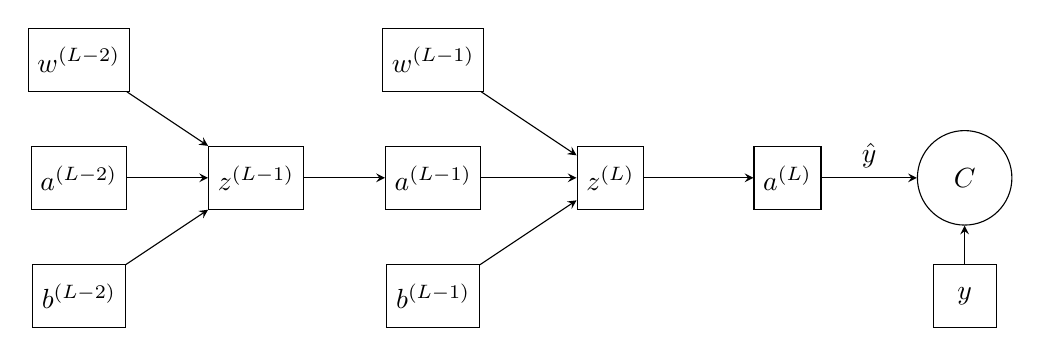
\begin{tikzpicture}[x=1.5cm, y=1.5cm,  >=stealth]
        \tikzstyle{unit}=[draw,shape=circle,minimum size=1.2cm]
        \tikzstyle{weight} =[draw, shape=rectangle, minimum size=.8cm]

        \node[weight](w-2) at (0, 2){$w^{(L-2)}$};
        \node[weight](a-2) at (0, 1){$a^{(L-2)}$};
        \node[weight](b-2) at (0,0){$b^{(L-2)}$};
        \node[weight](z-2) at (1.5, 1){$z^{(L-1)}$};
        \node[weight](w-1) at (3, 2){$w^{(L-1)}$};
        \node[weight](a-1) at (3, 1){$a^{(L-1)}$};
        \node[weight](b-1) at (3,0){$b^{(L-1)}$};
        \node[weight](z-1) at (4.5, 1){$z^{(L)}$};
        \node[weight](aL) at (6,1){$a^{(L)}$};
        \node[unit](c) at (7.5,1){$C$};
        \node[weight](y) at (7.5,0){$y$};

        \draw[->] (w-2) -- (z-2);
        \draw[->] (a-2) -- (z-2);
        \draw[->] (b-2) -- (z-2);
        \draw[->] (z-2) -- (a-1);
        \draw[->] (w-1) -- (z-1);
        \draw[->] (a-1) -- (z-1);
        \draw[->] (b-1) -- (z-1);
        \draw[->] (z-1) -- (aL);
        %\path [line] (aL) -- node [text width=2.5cm,midway,above ]{$\hat{y}$} (c);
        \draw[->] (aL) -> node [text width=2.5cm,midway,above,align=center ] {$\hat{y}$} (c);

        \draw[->] (y) -- (c);

        \end{tikzpicture}
    \caption[]{Explizite Darstellung Einflüsse der Verlustfunktion des gesamten Neural Networks}
    \label{fig:unfoldedCost2}
    Quelle: Eigene Darstellung, 2020
\end{figure}

Typischerweise haben \ac{NN} mehr als ein Neuron pro Layer, daher müssen die oben genannten Formeln noch leicht angepasst werden. In Gleichungen \ref{eq:forwardMulti} sind die Formeln für das Vorwärtsdurchlaufen des \ac{NN} dargestellt. Da nun mehrere Neuronen im Output Layer vorhanden sind - $N_L$ - muss über diese summiert werden. Anschließend muss für den quadratischen Mittelwert noch durch die Anzahl der Neuronen geteilt werden (siehe Formel 1 in Abbildung \ref{eq:forwardMulti}).

Auch die gewichtet Summe in jedem Neuron hängt nun von allen Aktivierungen des vorherigen Layer ($N_{(L-1)}$) ab, so dass hier ebenfalls über diese summiert werden muss. Da es nun mehrere Neuronen pro Layer - und somit mehrere gewichtete Summen pro Layer - gibt, wird mittels dem Index  $j$ noch spezifiziert, welches Neuronen gerade berechnet wird.

\begin{equation} \label{eq:forwardMulti}
    \begin{split}
        &C=\frac{1}{N_{L}} \sum_{j=1}^{N_{L}}\left(a_{j}^{(L)}-y_{j}\right)^{2} \\
        &z_{j}^{(L)}=\sum_{k=1}^{N_{L-1}} w_{j k}^{(L-1)} a_{k}^{(L-1)}+b_{j}^{(L-1)} \\
        &a_{j}^{(L)}=\sigma\left(z_{j}^{(L)}\right)
    \end{split}
\end{equation}


Wendet man die gleiche Vorgehensweise und Überlegung wie für das des einfachen \ac{NN} an und nutzt zusätzlich die neue Notation, erhält man für den Einfluss das Gewichtes $w_{j k}^{(L-1)}$ Gleichung \ref{eq:infWLayer1}. Ähnlich wie beim einfachen \ac{NN} unterscheidet sich die Formel für ein Bias nur durch die geänderten Formelzeichen, daher wird auf eine explizite Darstellung verzichtet.


\begin{equation} \label{eq:infWLayer1}
    \frac{\partial C}{\partial w_{j k}^{(L-1)}}=\frac{\partial z_{j}^{(L)}}{\partial w_{j k}^{(L-1)}} \frac{\partial a_{j}^{(L)}}{\partial z_{j}^{(L)}} \frac{\partial C}{\partial a_{j}^{(L)}}
\end{equation}

Größere Änderungen gibt es für den Einfluss der Aktivierung $a_{k}^{(L-1)}$. Da jedes Neuron in diesem Hidden Layer mit jedem Neuron im Output Layer verbunden ist, hat es auch Einfluss auf den Fehler jedes Neurons im Output Layer. Möchte man also den gesamten Fehler eines Neurons im Hidden Layer berechnen, muss man die Summe über alle zurückgeführten Fehler aus dem Output Layer bilden (siehe Gleichungen \ref{eq:infALayer1}).

\begin{equation} \label{eq:infALayer1}
        \frac{\partial C}{\partial a_{k}^{(L-1)}}=\sum_{j=1}^{N_{L}} \frac{\partial z_{j}^{(L)}}{\partial a_{k}^{(L-1)}} \frac{\partial a_{j}^{(L)}}{\partial z_{j}^{(L)}} \frac{\partial C}{\partial a_{j}^{(L)}} \\
\end{equation}

Neben dem hinzufügen der neuen Notation mit Indizes und der Summe, gibt es keine Änderungen zum Fall im einfachen \ac{NN}. Dies lässt sich auch beobachten, wenn ein weiteren Schritt zurück Gegangen wird. Also Elemente im Layer $L-2$ betrachtet werden. Für das Gewicht $w_{j k}^{(L-2)}$ wird die Formel in Gleichung \ref{eq:infWL-2} dargestellt. Genau wie beim einfachen \ac{NN}, wurde das Ergebnis des vorherigen Layers um zwei weitere Terme ergänzt. Ähnlich sieht es bei der Aktivierung aus, hier enthält der letzte Term in Summenzeichen aus Gleichung \ref{eq:infALayer1} immer den Weg vom aktuellen Layer bis zu $C$, so dass die zwei anderen Terme in der Summe nur auf den aktuellen Layer angepasst werden müssen. 

\begin{equation} \label{eq:infWL-2}
    \frac{\partial C}{\partial w_{j k}^{(L-2)}}=\frac{\partial z_{j k}^{(L-1)}}{\partial w_{j k}^{(L-2)}} \frac{\partial a_{j}^{(L-1)}}{\partial z_{j}^{(L-1)}} \frac{\partial C}{\partial a_{j}^{(L-1)}}
\end{equation}

Verwendet man die hergeleiteten Gleichungen und erweitert sie gegebenenfalls für weitere Hidden Layer, ist man in der Lage die Anpassungen aller Gewichte und Bias in einem \ac{NN} zu berechnen. Der komplette Lernprozess besteht dann aus den folgenden vier Schritten:

\begin{enumerate}
    \item Durchführen eines Vorwärtsdurchlaufs um die Ausgabe des Output Layers zu erhalten (\textit{\^{y}})
    \item Ausrechnen der Verlustfunktion ($C(w,b)$), um den Fehler des \ac{NN} zu erhalten
    \item Berechnen der Gradienten von $C(w,b)$ im Bezug auf alle Gewichte und Bias im \ac{NN}
    \item Anpassen der Gewichte und Bias im Netzwerk anhand der berechneten Gradienten und den Ausgangswerte
\end{enumerate}
\subsection{Convolutional Neural Networks} \label{sec:CNN}
Wie bereits dargestellt, sind alle Neuronen in einem \ac{NN} miteinander verbunden. Dies führt dazu, dass die Zahl der Parameter innerhalb des \ac{NN} schnell steigen kann. Dies ist zum Beispiel bei Bildern, bei denen jeder einzelne Pixel ein eigenen Eingabewert in das Netzwerk darstellt, der Fall. Da für jeden Parameter Berechnungen durchgeführt werden müssen, skalieren \ac{NN} dementsprechend schlecht.

Zusätzlich entstehen Formen und Objekte in Bildern erst durch den räumlichen Zusammenhang einiger Pixel. Daher erscheint das Vorgehen, alle Neuronen im Input Layer (Pixelwerte) mit allen Neuronen im ersten Hidden Layer zu verbinden, als wenig sinnvoll.

Aus diesen und weiteren Gründen, werden heutzutage \ac{CNN} für die Klassifizierung von Bildern verwendet. Durch besondere Bausteine sorgen diese dafür, dass sowohl der räumliche Zusammenhang der Pixel betrachtet wird, als auch die Anzahl von Parametern besser skalierbar ist. Basierend auf den biologischen Vorbildern - siehe nächster Abschnitt - schlugen Fukushima und Miyake im Jahre 1972 \textit{Neocognitron} vor, welches als ein Vorgänger von \ac{CNN} gesehen werden kann.\footcite[Vgl.][S. 267–285]{fukushima1982neocognitron} LeCun et. al verwendeten in ihrem Artikel \textit{Handwritten digit recognition with a back-propagation network} von 1990 einem dem \textit{Convolutional Layer} (siehe Abschnitt \ref{LocalReceptiveFields}) ähnlichen Aufbau.\footcite[Vgl.][S. 396–404]{lecun1990handwritten} Der Artikel \textit{Gradient-based learning applied to document recognition} von LeCun et. al aus dem Jahre 1998 beschreibt das erste Mal den Aufbau eines heute üblichen \ac{CNN}.\footcite[Vgl.][S. 2278–2324]{lecunGradientbasedLearningApplied1998}

\subsubsection{Biologische Grundlagen}
\ac{CNN} basieren auf Beobachtungen der Funktionsweise des visuellen Cortex bei Menschen und Tieren. So haben Hubel und Wiesel 1959 bzw. 1962 gezeigt, das einzelne Sehzellen nur auf Veränderungen in einzelnen Bereichen der Netzhaut reagieren. Dieses Bereiche wurden von Hubel und Wiesel als \textit{receptive field} bezeichnet. \footcite[Vgl. ][S. 574-591]{hubelReceptiveFieldsSingle1959} \footcite[Vgl. ][S. 106-154]{hubelReceptiveFieldsBinocular1962}


\todo{Verweis 13,14 Masterthesis}

\begin{figure}[t]
    \centering
    \caption[]{Vereinfachter Aufbau visueller Cortex und \ac{CNN}}
	\label{fig:humVisVsCNN}
    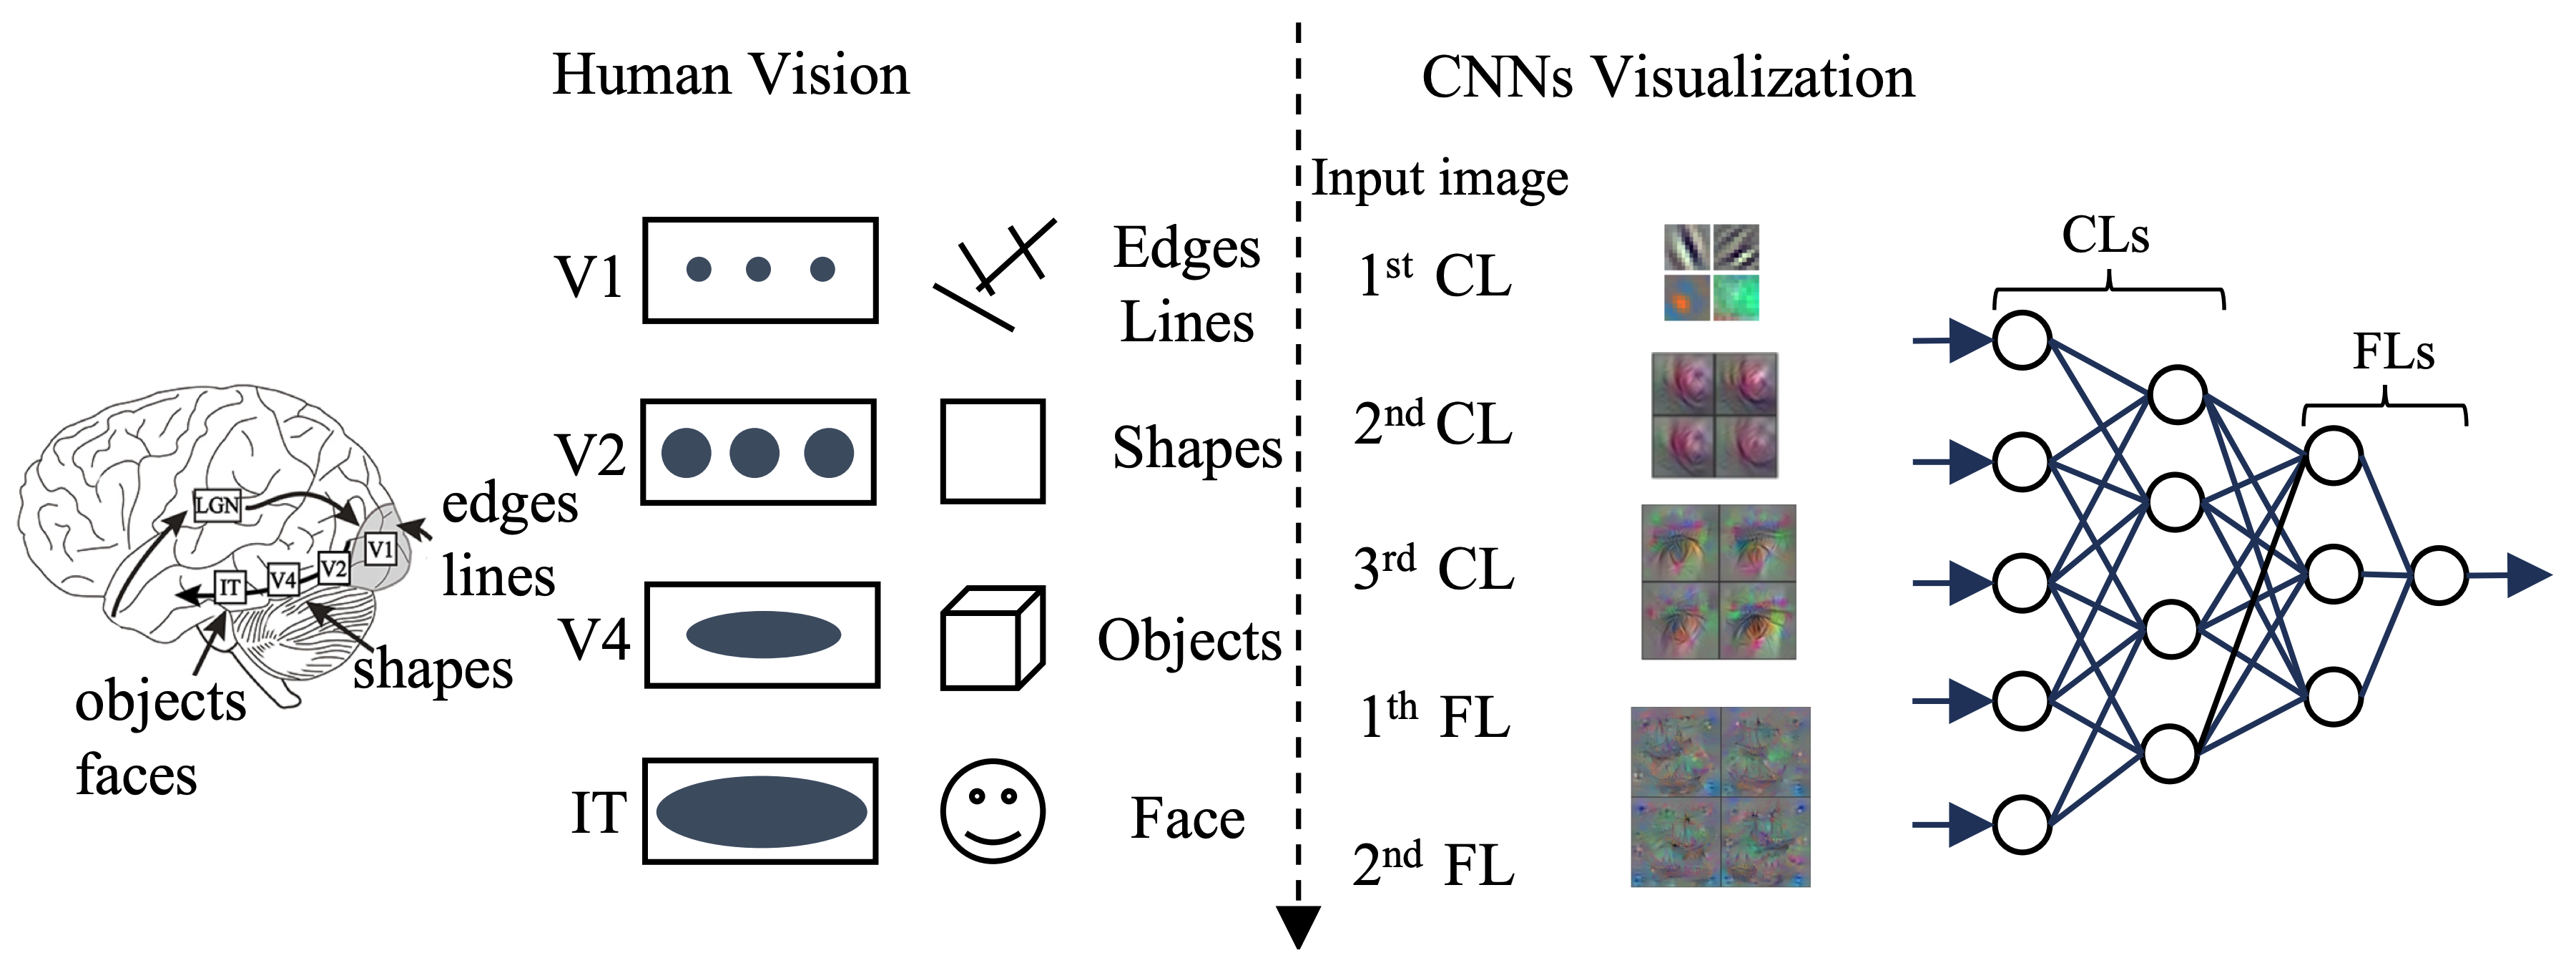
\includegraphics[width=1\textwidth]{human_vis_vs_cnn.png}
    Quelle: Qin et al., 2018
\end{figure}

In Abbildung \ref{fig:humVisVsCNN} wird der vereinfachte visuell Cortex eines Menschen dem Aufbau eines \ac{CNN} gegenübergestellt. Auf der linken Seite ist zu erkennen, dass beim visuellen Cortex verschiedene Schichten (V1, V2, V4 und IT) vorliegen, welche nacheinander geschaltet sind. Jede dieser Schichten enthält \textit{receptive fields}, wobei diese mit jeder Schicht größer werden. Die früheren Schichten reagieren hierbei auf einfache Formen wie Linien oder Kanten und die späteren auf komplexere Formen wie ganze Objekte. Bei allen Schichten können die gesamten Elemente an jeder Stelle des \textit{receptive field} auftreten und trotzdem für eine Aktivierung sorgen. Die rechte Seite zeigt den typischen Aufbau eines \ac{CNN}, bei dem die früheren Schichten (CL) einfache und spätere Schichten (FL) komplexe Formen erkennen. \footcite[Vgl. ][S. 6]{qinHowConvolutionalNeural2018}

\subsubsection{Architektur}
\ac{CNN} haben drei grundlegende Ideen bzw. Bausteine, die sie von anderen \ac{NN} unterscheiden. Diese sind \textit{\ac{LRF}}, \textit{gemeinsame Gewichte und Bias} sowie \textit{Pooling} und werden in diesem Abschnitt genauer beleuchtet.

\paragraph{Local Receptive Fields} \label{LocalReceptiveFields}
Die Grundidee hinter \ac{LRF} ist - ähnlich wie mein visuellen Cortex - Neuronen zu erzeugen, die in bestimmte Bereiche auf Formen reagieren. Anders gesagt, sollen die einzelnen Neuronen einen Teil des Bildes betrachten und hier Formen erkennen können. Stellt man sich das Eingangssignal als Matrix statt einem Vektor vor, lässt sich das ganze einfacher visualisieren. Ein Bild mit 28x28 Pixel entspricht also einer 28x28 Matrix, siehe Abbildung \ref{fig:lrf} links. Um nun die \ac{LRF} nachzubilden, wird eine kleinere Matrix - typischerweise als \textit{Filter} oder \textit{Kernel} bezeichnet - über das Bild geschoben. Typische Maße für den Kernel sind hierbei 3x3, 4x4 oder 5x5. Alle Pixel die vom Kernel übereckt werden, werden in der Berechnung für den Pixelwert in der Ausgabe zusammengefasst (siehe Abbildung \ref{fig:lrf} rechts). Bei einer Matrix mit den Maßen 5x5 bedeutet dies, dass ein Pixel in der Ausgabe 25 Werte zusammenfasst. Die Werte innerhalb der Kernel-Matrix stellen dabei die Gewichte für jeden einzelnen Pixel dar. Zusätzlich hat jeder Pixel in der Ausgabe auch noch einen eigenen Bias.

Wandert der Kernel über das Bild, kann er um \textit{n} Schritte nach rechts bzw. um \textit{m} Schritte nach unten verschoben werden. Hierdurch wird bestimmt, welche Pixel in der Ausgabe zusammengefasst werden. Diese Schrittweite wird als \textit{Stride} bezeichnet. Betrachtet man ein Bild mit 28x28 Pixeln, einen 5x5 Kernel und einen Stride von 1, besteht die Ausgabe aus 24x24 Pixeln. Dies liegt daran, dass man den Kernel von der Ausgangsposition nur 23 Mal um eins nach rechts bzw. unten schieben kann. Um zu verhindern, dass die Matrix im nachfolgendem Layer kleiner wird, kann \textit{Padding} angewendet werden. Hierbei werden um das Bild herum weitere Pixel ergänzt. Typischerweise geschieht dies symmetrisch, allerdings ist es auch möglich unterschiedlich viele Reihen auf jeder Seite hinzuzufügen. Der Wert der hinzugefügten Pixel wird typischerweise auf $0$ gesetzt.

Die Anzahl der Spalten in der Ausgabe kann mit Gleichung \ref{eq:CalcOutputSize} berechnet werden.\footcite[Vgl.][S. 15]{dumoulinGuideConvolutionArithmetic2018} Hierbei steht $i$ für die Anzahl der Spalten in der Matrix die das ursprüngliche Bild darstellt, $p_{links}$ für die Anzahl von Spalten die durch das Padding links hinzugefügt wurden ($p_{rechts}$ dementsprechend für die rechts), $k$ für die Maße des Kernels und $s$ für den Stride. Sind das Bild und der Kernel quadratisch und durch Padding wurde an allen Seiten gleich viele Spalten hinzugefügt, entspricht das Ergebnis auch der Anzahl an Zeilen in der Ausgabe. \footcite[Vgl.][S. 169-171]{nielsenNeuralNetworksDeep2015}

\begin{equation} \label{eq:CalcOutputSize}
    o=\left\lfloor\frac{i+p_{links}+p_{rechts}-k}{s}\right\rfloor+1
\end{equation}


\begin{figure}[t]
    \centering
    \caption[]{Input Layer als Matrix (links) und Beispiel \ac{LRF} zwischen Input und 1. Hidden Layer}
	\label{fig:lrf}
    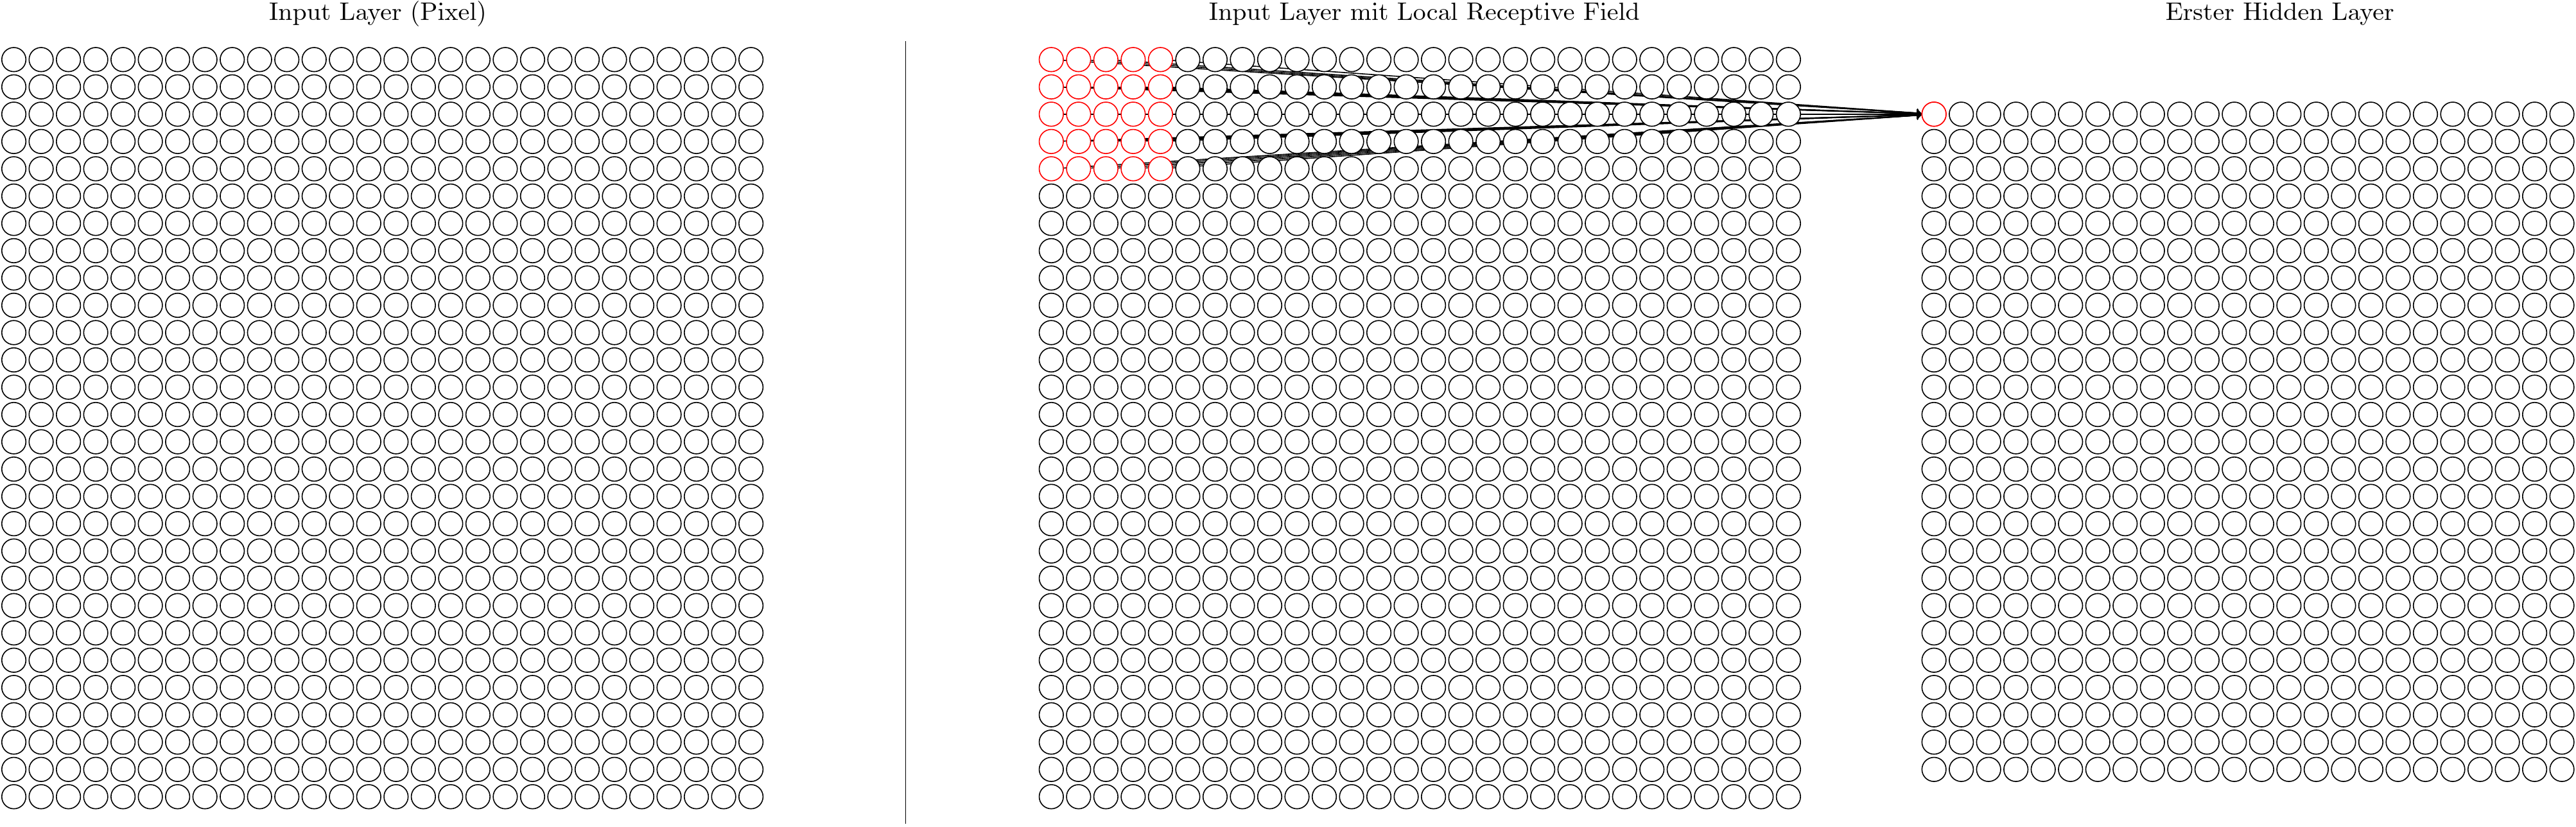
\includegraphics[width=1\textwidth]{lrf.png}
    Quelle: In Anlehnung an Nielsen, Introduction CNN, 2018, S. 170 f.
\end{figure}

\paragraph{Gemeinsame Gewichte und Bias}
Wie bereits erwähnt, stellen die Werte der Kernel-Matrix die Gewichte für jeden einzelnen Pixel im Bild dar. Allerdings werden außerdem die gleichen Werte innerhalb des Kernels für alle Verschiebungen verwendet. Bei einem 28x28 Layer und einer 5x5 Matrix, werden also alle 24x24 Pixel im Ausgang mit den gleichen Gewichten und Bias berechnet (siehe Gleichung \ref{eq:actSharedWeights}).

\begin{equation}
    \label{eq:actSharedWeights}
    pixel_{j,k} = \sigma\left(b+\sum_{l=0}^{z} \sum_{m=0}^{s} w_{l, m} a_{j+l, k+m}\right)
\end{equation}

Hierbei steht ($z$) für die Anzahl der Zeilen und $s$ für die Anzahl von Spalten der Matrix des Bildes. $b$ ist der gemeinsame Bias, $w$ das Gewicht an Position $l,m$ der Matrix und $a$ der Wert innerhalb des Kernels. Typischerweise wird die berechnete Summe noch in eine Aktivierungsfunktion gegeben, welche durch $\sigma$ dargestellt wird.

Das bedeutet, dass durch den Kernel überall auf dem Bild die gleichen Formen beziehungsweise Objekte erkannt werden. Man stelle sich zum Beispiel vor, dass der Kernel durch das Anpassen seiner Gewichte gelernt hat vertikale Linien zu erkennen. Dann ist es sinnvoll, dass diese vertikale Linie überall auf dem Bild erkannt werden kann. Genau dies wird durch die gemeinsamen Gewichte und Bias erreicht.

Das Element, auf welches ein Kernel reagiert, wird als \textit{Feature} bezeichnet. Daher werden die Matrizen in der Ausgabe auch \textit{Feature Maps} genannt. Insgesamt wird ein Layer in einem \ac{CNN}, welcher Feature Maps mit gemeinsamen Gewichten anwendet, als \textit{Convolutional Layer} bezeichnet. Ein \ac{CNN} soll mehr als ein Feature pro Convolutional Layer erkennen können. Daher können pro Convolutional Layer $n$ verschiedene Kernels verwendet werden. Mit jedem Kernel ensteht eine neue Matrix in der Ausgabe. Die Ausgabe stellt somit eine dreidimensionale Matrix dar, bildlich gesehen kann man sich einen Stapel von zweidimensionalen Matrizen vorstellen (siehe Convolution Layer in \ref{fig:convAndPool}).
Grundsätzlich reagieren Kernels in Convolutional Layern die früh im \ac{CNN} vorkommen eher auf einfache Formen wie Kanten oder Ecken. Später reagieren Convolutional Layer dann auf komplexere Formen bzw. Objekte. Auf der rechten Seite in Abbildung \ref{fig:humVisVsCNN} ist dies dargestellt. Währen im ersten CL Layer einfache Linien erkannt werden, kann man im dritten CL Layer bereits Augen erkennen.\footcite[Vgl.][S. 169-171]{nielsenNeuralNetworksDeep2015}

\paragraph{Pooling}
Neben dem beschriebenen Convolutional Layer, haben \ac{CNN} eine weitere besonderen Layer. Dieser wird als \textit{Pooling Layer} bezeichnet und typischerweise direkt hinter einem Convolutional Layer angewendet. 

Ein Pooling Layer vereinfacht hierbei die vorliegenden Informationen, also die Matrizen die der vorherige Layer ausgegeben hat. Folgt der Pooling Layer auf einen Convolutional, sind dies die Ausgaben der Feature Maps, also die Werte, die durch die Berechnung der Aktivierungsfunktion erhalten werden.

Beim Pooling werden mehrere Werte zusammengefasst, es wird also erneut eine Art Filter (Quadrat) über die Matrix gelegt und alle überdeckten Werte werden zusammen betrachtet. Am verbreitesten sind hierbei das \textit{Max Pooling} und das \textit{Average Pooling}. Wie durch die Namen zu erkennen, wird beim Max Pooling der maximale Wert innerhalb der betrachteten Werte verwendet, während beim Average Pooling der Durchschnitt berechnet wird. Beides ist in Abbildung \ref{fig:pooling} beispielhaft dargestellt. Die Maße der Matrix verändern sich entsprechend der gewählten Filter Matrix, bei einer 2x2 Matrix wird die Anzahl der Spalten und Zeilen halbiert.
Das Pooling wird hierbei auf jede Feature Map separat angewendet, die Anzahl der Matrizen ändert sich also nicht. 

Durch Pooling wird geprüft, ob ein Element durch den Convolutional Layer gefunden wurde (= hohe Werte). Die Grundannahme geht hierbei davon aus, dass die Information das dieses Element vorhanden ist, aber nicht die genaue Position relevant ist. Durch das Pooling bleibt die Information erhalten, nur die Genauigkeit der Positionsangabe sinkt. Hierfür wird wiederum die Anzahl der Parameter stark reduziert. 

In Abbildung \ref{fig:convAndPool} ist der Beginn eines \ac{CNN} dargestellt. Hier wird ein Convolutional Layer als erster Hidden Layer verwendet und dessen Ausgabe (Feature Maps) werden als Input für den Pooling Layer (zweiter Hidden Layer) verwendet. Dessen Ausgabe wird in einen Dense Layer gegeben, also einem Layer der mit allen Neuronen des vorherigen Layers verbunden ist.\footcite[Vgl.][S. 169-171]{nielsenNeuralNetworksDeep2015}

\begin{figure}[t]
    \centering
    \begin{tikzpicture}[x=1.5cm, y=1.5cm,  >=stealth]
        \tikzset{square matrix/.style={
            matrix of nodes,
            column sep=-\pgflinewidth, row sep=-\pgflinewidth,
            nodes={draw,
            text height=#1/2+0.75ex,
            text depth=#1/2-0.75ex,
            text width=#1,
            align=center,
            inner sep=0pt
            },
        },
        square matrix/.default=1.4cm
        }

        \matrix[square matrix](matrix)
        {
            |[fill=lightgray]|163 & |[fill=lightgray]|131 &0 & 42   \\
            |[fill=lightgray]|248 & |[fill=lightgray]|247 & 161 & 89  \\
            || 13 & 120 & 62 & 8 \\
            || 40 & 19 & 23 & 168 \\
        };

        \node[text width=6cm] at (5, 1) 
            {\baselineskip=25pt \underline{\textbf{Max Pooling:}} \\ $max(163, 131, 248, 247) = 248$ \par};

        \node[text width=6cm] at (5, -1) 
            {\baselineskip=25pt \underline{\textbf{Average Pooling:}} \\ $\frac{163 + 131 + 248 + 247}{4} = 197$ \par};
        
    \end{tikzpicture}
    \caption[]{Beispiel Max Pooling und Average Pooling}
    \label{fig:pooling}
    Quelle: Eigene Darstellung, 2020
\end{figure}

\begin{figure}[t]
    \centering
    \caption[]{Convolutional und Pooling Layer im Zusammenspiel}
	\label{fig:convAndPool}
    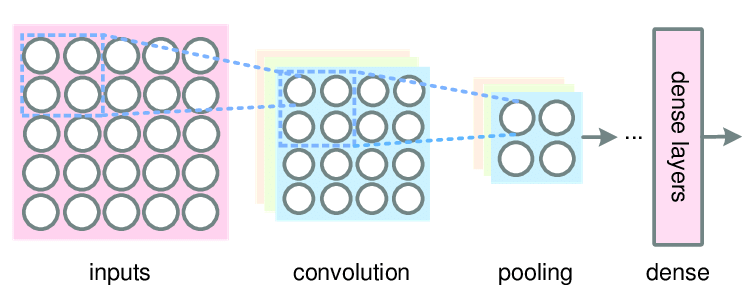
\includegraphics[width=1\textwidth]{overview_cl_pooling.png}
    Quelle: Wang et. al, Wireless Layer, 2017, S. 4
\end{figure}

\subsection{Visualisierung der Entscheidung} \label{sec:visAlgos}

\subsubsection{Activation Maximaztion} \label{sec:actMax}
% https://github.com/MisaOgura/flashtorch


% Misa Ogura, & Ravi Jain. (2020, January 2).
% MisaOgura/flashtorch: 0.1.2 (Version v0.1.2).
% Zenodo. http://doi.org/10.5281/zenodo.3596650


\subsubsection{Backpropagation} \label{sec:backprop}
% J. T. Springenberg, A. Dosovitskiy, T. Brox, and M. Riedmiller. Striving for Simplicity: The All Convolutional Net, https://arxiv.org/abs/1412.6806

% Entweder vanilla oder saliency....

% code: https://github.com/utkuozbulak/pytorch-cnn-visualizations
% @misc{uozbulak_pytorch_vis_2019,
%   author = {Utku Ozbulak},
%   title = {PyTorch CNN Visualizations},
%   year = {2019},
%   publisher = {GitHub},
%   journal = {GitHub repository},
%   howpublished = {\url{https://github.com/utkuozbulak/pytorch-cnn-visualizations}},
%   commit = {47c6cd2121b4d0bcbe76f63abe9e13c5fb1ea0ff}
% }

\subsubsection{Gradient-weighted class activation mapping}
% B. Zhou, A. Khosla, A. Lapedriza, A. Oliva, A. Torralba. Learning Deep Features for Discriminative Localization, https://arxiv.org/abs/1512.04150

% R. R. Selvaraju, A. Das, R. Vedantam, M. Cogswell, D. Parikh, and D. Batra. Grad-CAM: Visual Explanations from Deep Networks via Gradient-based Localization, https://arxiv.org/abs/1610.02391

% code: https://github.com/utkuozbulak/pytorch-cnn-visualizations
% @misc{uozbulak_pytorch_vis_2019,
%   author = {Utku Ozbulak},
%   title = {PyTorch CNN Visualizations},
%   year = {2019},
%   publisher = {GitHub},
%   journal = {GitHub repository},
%   howpublished = {\url{https://github.com/utkuozbulak/pytorch-cnn-visualizations}},
%   commit = {47c6cd2121b4d0bcbe76f63abe9e13c5fb1ea0ff}
% }
\section{Bibliotheken} \label{sec:bibs}